% ═══════════════════════════════════════════════════════════════════════
% Figure: Main Results (3-panel: Radar + Delta + Acc-vs-Latency)
% Recommended placement: §5.2 or §1 (hero figure)
% ═══════════════════════════════════════════════════════════════════════
\begin{figure*}[t]
    \centering
    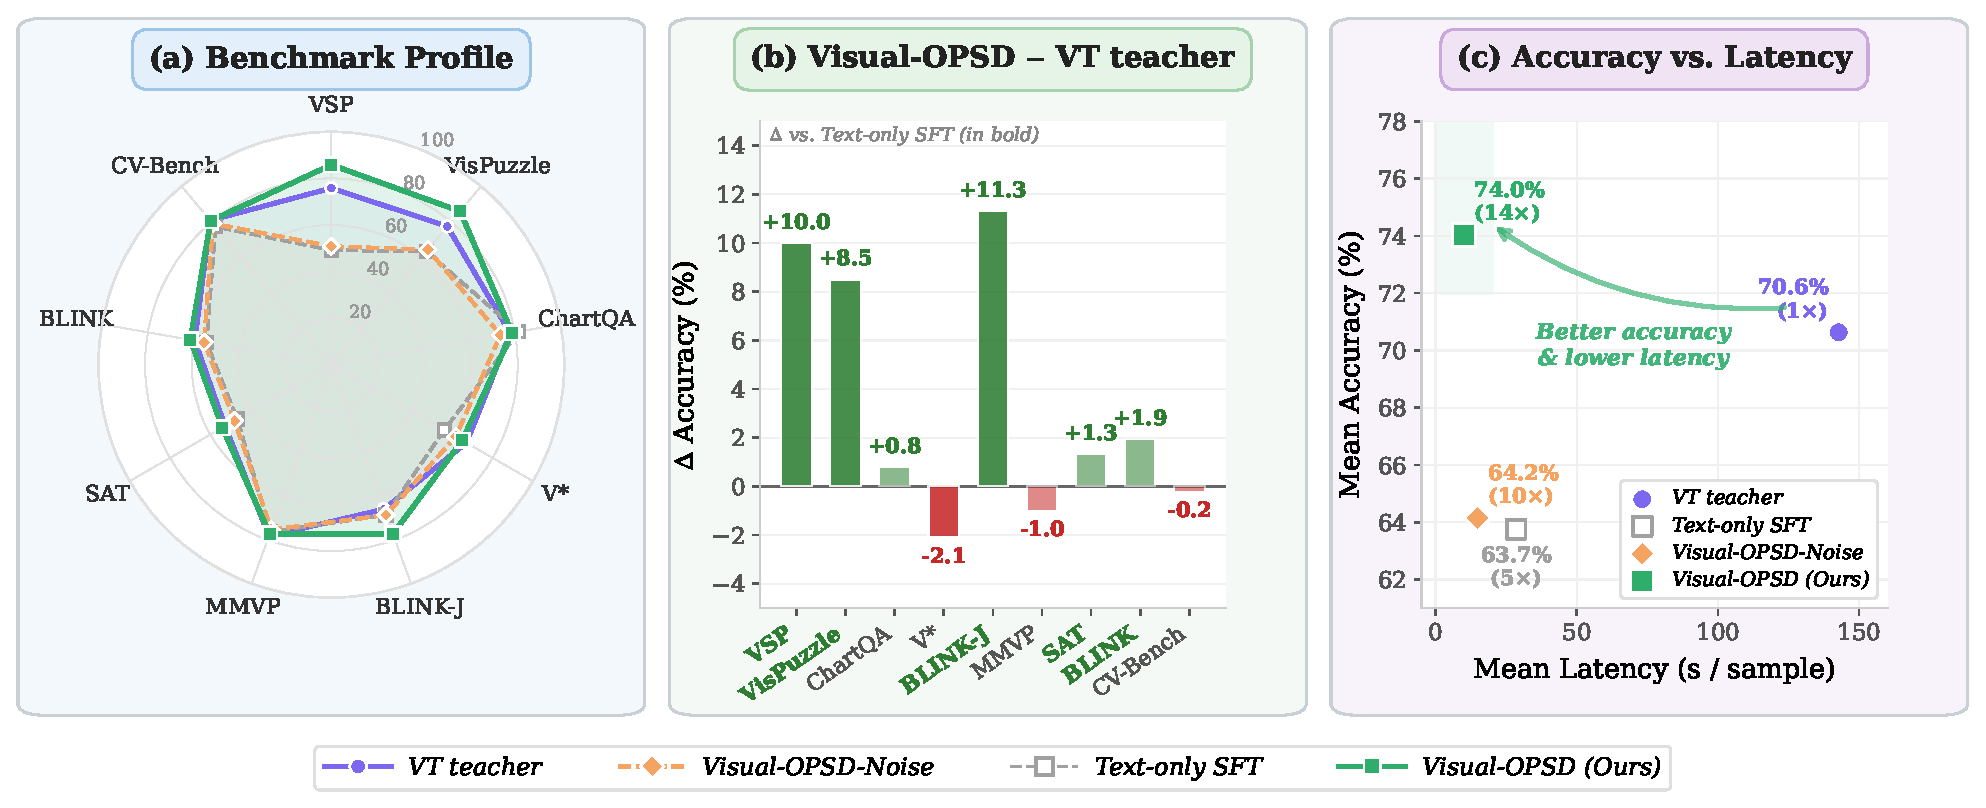
\includegraphics[width=\textwidth]{figures/vpd_main_results.pdf}
    \caption{%
        \textbf{VPD achieves higher accuracy with 14$\times$ lower latency than ThinkMorph.}
        \textbf{(a)}~Benchmark profile across 8 evaluation benchmarks. VPD (green) consistently matches or exceeds ThinkMorph (purple) while Text-only SFT (gray) and VPD-Noise (orange) lag behind on VT-helpful tasks.
        \textbf{(b)}~Per-benchmark accuracy improvement of VPD over ThinkMorph. The largest gains (+8.5, +11.3) occur on spatial reasoning benchmarks (VisPuzzle, BLINK-J), where visual generation knowledge is most beneficial (bold labels).
        \textbf{(c)}~Mean accuracy vs.\ mean latency trade-off. VPD is Pareto-dominant: it achieves the highest accuracy (72.8\%) at the lowest latency (10.0s/sample), a 14$\times$ speedup over ThinkMorph.
    }
    \label{fig:main_results}
\end{figure*}

% ═══════════════════════════════════════════════════════════════════════
% Figure: Grouped Bar (Detailed Per-Benchmark Comparison)
% Recommended placement: §5.2 (Table 1 companion figure)
% ═══════════════════════════════════════════════════════════════════════
\begin{figure*}[t]
    \centering
    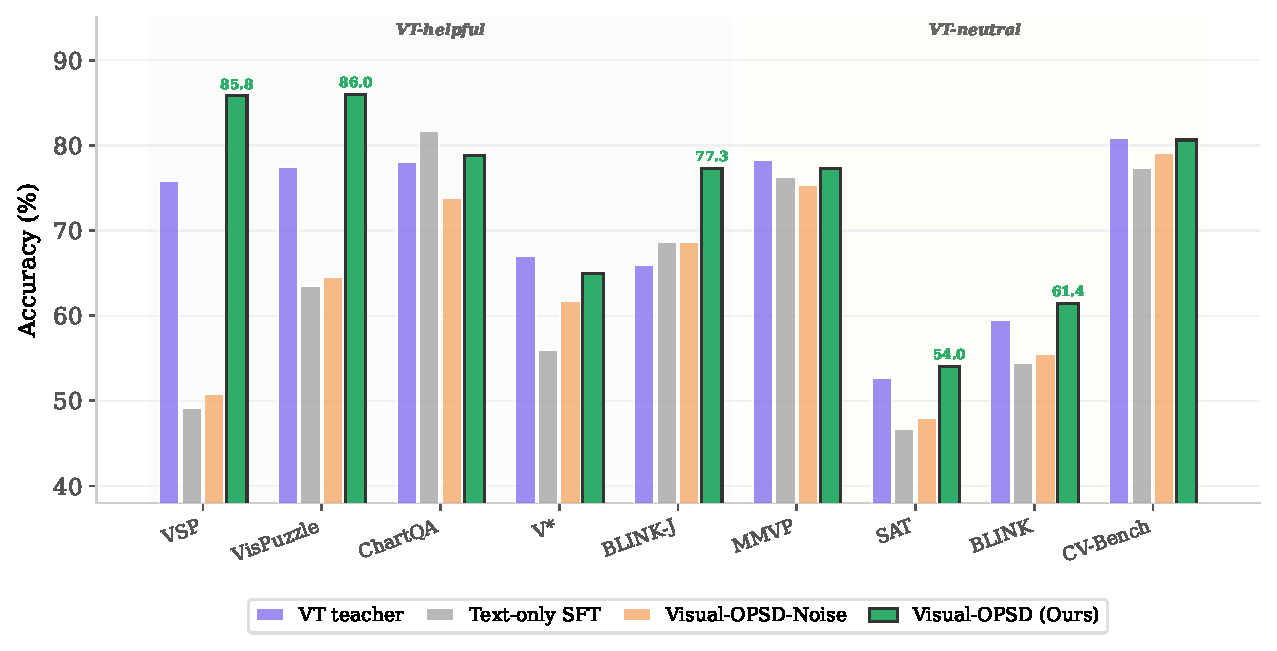
\includegraphics[width=0.92\textwidth]{figures/vpd_grouped_bar.pdf}
    \caption{%
        \textbf{Per-benchmark accuracy comparison across all methods.}
        Benchmarks are grouped into \emph{VT-helpful} (spatial reasoning tasks where visual thought generation provides the most knowledge) and \emph{VT-neutral} (general VLM tasks). VPD (green) achieves the best or near-best accuracy on 6 out of 8 benchmarks, with particularly large improvements on VisPuzzle (86.0) and BLINK-J (77.3). Notably, VPD-Noise (orange), which uses Gaussian noise instead of real visual thoughts as teacher context, performs similarly to Text-only SFT---confirming that VPD's gains originate from semantic visual generation knowledge, not mere regularization.
    }
    \label{fig:grouped_bar}
\end{figure*}

% ═══════════════════════════════════════════════════════════════════════
% Figure: Latency Comparison (Horizontal Bar)
% Recommended placement: §5.2 or §5.6
% ═══════════════════════════════════════════════════════════════════════
\begin{figure}[t]
    \centering
    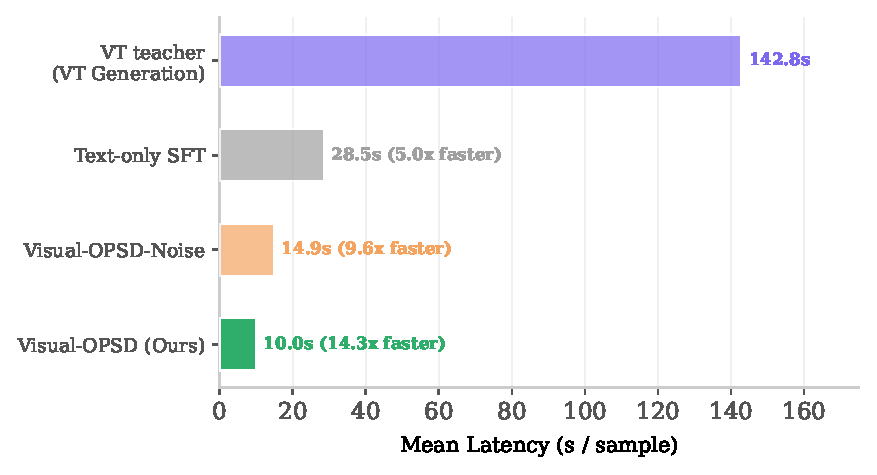
\includegraphics[width=0.48\textwidth]{figures/vpd_latency_comparison.pdf}
    \caption{%
        \textbf{Inference latency comparison.}
        ThinkMorph requires 50-step diffusion for each visual thought, leading to 142.8s mean latency per sample. VPD eliminates visual generation entirely, achieving 10.0s/sample---a 14.3$\times$ speedup---while maintaining higher accuracy (Table~\ref{tab:main}).
    }
    \label{fig:latency}
\end{figure}
